% =============================================================================
%  Medical Imaging AI -- Proje Analiz Raporu
%  IEEE konferans sablonu (IEEEtran). Turkce karakterler icin babel YERINE
%  inputenc + fontenc kullaniliyor; babel'in [turkish] secenegi figure
%  scaling ile catismaktadir.
% =============================================================================
\documentclass[conference]{IEEEtran}

\IEEEoverridecommandlockouts

% ---- Encoding & fonts (babel/turkish KULLANILMIYOR) ------------------------
\usepackage[utf8]{inputenc}
\usepackage[T1]{fontenc}
\usepackage{lmodern}

% ---- Math, tables, graphics, code -----------------------------------------
\usepackage{amsmath,amssymb,amsfonts}
\usepackage{graphicx}
\usepackage{booktabs}
\usepackage{array}
\usepackage{tabularx}
\usepackage{multirow}
\usepackage{caption}
\usepackage{subcaption}
\usepackage{listings}
\usepackage{xcolor}
\usepackage{url}
\usepackage{hyperref}
\usepackage{textcomp}

% ---- Listings tasarimi (kod bloklari icin) --------------------------------
\definecolor{codegray}{rgb}{0.95,0.95,0.95}
\definecolor{codekey}{rgb}{0.0,0.0,0.6}
\definecolor{codestr}{rgb}{0.6,0.0,0.0}
\definecolor{codecmt}{rgb}{0.25,0.5,0.25}
\lstset{
  backgroundcolor=\color{codegray},
  basicstyle=\ttfamily\footnotesize,
  keywordstyle=\color{codekey}\bfseries,
  stringstyle=\color{codestr},
  commentstyle=\color{codecmt}\itshape,
  breaklines=true,
  showstringspaces=false,
  frame=single,
  rulecolor=\color{black!20},
  columns=fullflexible,
  upquote=true,
  literate=%
    {ç}{{\c{c}}}1 {ı}{{\i}}1 {ğ}{{\u{g}}}1
    {ö}{{\"o}}1 {ş}{{\c{s}}}1 {ü}{{\"u}}1
    {Ç}{{\c{C}}}1 {İ}{{\.I}}1 {Ğ}{{\u{G}}}1
    {Ö}{{\"O}}1 {Ş}{{\c{S}}}1 {Ü}{{\"U}}1
}

\hypersetup{
  colorlinks=true,
  linkcolor=blue!60!black,
  citecolor=blue!60!black,
  urlcolor=blue!60!black
}

% Tireleme: Turkce icin temel ozel durumlar (babel yok, manuel)
\hyphenation{seg-men-tas-yon sınıf-lan-dır-ma rad-yo-loji}

\begin{document}

% =============================================================================
\title{Beyin MR Tumor Segmentasyonu ve Akciger X-Ray Patoloji Siniflandirmasi
icin Hibrit Bir Derin Ogrenme Cercevesi: BraTS 2020 ve COVID-19 Radiography
Veri Setleri Uzerinde Atension U-Net ve DenseNet-121 Tabanli Bir Uygulama}

\author{\IEEEauthorblockN{Barbaros Umut}
\IEEEauthorblockA{\textit{Tibbi Goruntuleme Yapay Zeka Projesi} \\
\textit{Bireysel Calisma}\\
GitHub: \url{https://github.com/BarbarosUmut/Medical_Imaging_Ai}\\
E-posta: umutbarbarosbaba@gmail.com}
}

\maketitle

% =============================================================================
\begin{abstract}
Bu rapor, beyin MR goruntulerinde tumor segmentasyonu ve gogus rontgenlerinde
patoloji siniflandirmasi yapan, sonuclari Ollama tabanli bir yerel buyuk dil
modeli ile Turkce klinik radyoloji raporuna doken Gradio tabanli bir
uygulamanin tasarimini, egitim surecini ve elde edilen sonuclari aktarir.
Segmentasyon icin BraTS 2020 veri seti uzerinde MONAI cercevesi ile bir 2B ve
bir 3B Attention U-Net egitilmis, siniflandirma icin COVID-19 Radiography
Database uzerinde DenseNet-121 mimarisi ImageNet on egitimi ile ince
ayarlanmistir. En iyi konfigurasyonlarda 2B model 0.827, 3B model 0.764
ortalama Dice; akciger modeli ise dogrulamada \%95.9 dogruluk ve 0.963 makro
F1 skoruna ulasti. Calismada hangi yontemlerin ise yaradigi kadar hangilerinin
basarisiz oldugu da ele aliniyor; sade U-Net ile baslayip Attention bloklarinin
eklenmesi, lung tarafinda MixUp/CutMix denemelerinin geri cevrilmesi ve
warm-up'li bir ogrenme orani plani uygulanmasi gibi degisiklikler ardisik
denemelerle netlesti. Sistem nihayetinde tek bir Windows yurutulebilirine
paketlenerek \texttt{.exe} formatinda yayinlandi; bu rapor ayrica calistirma
talimatlarini, dosya formati kisitlamalarini ve literaturden ilham alan
gelistirme onerilerini de iceriyor.
\end{abstract}

\begin{IEEEkeywords}
tibbi goruntu segmentasyonu, beyin tumoru, BraTS, U-Net, Attention U-Net,
DenseNet, COVID-19, gogus rontgeni, MONAI, Ollama, Gradio, Grad-CAM
\end{IEEEkeywords}

% =============================================================================
\section{Giris}

Tibbi goruntu yorumlamasi, hem zaman alici hem de yorumlayicilar arasinda
degiskenlige acik bir surec olmaya devam ediyor. Ozellikle ileri merkezler
disinda gorev yapan klinisyenler icin, MR ve rontgen gibi modaliteler uzerinde
hizli ve tutarli bir on-degerlendirme sunan yardimci araclara olan ilgi son
yillarda belirgin sekilde arti. Bu rapor, bu motivasyondan hareketle
gelistirilen yerel ve cevrimdisi calisabilen bir tibbi goruntuleme yapay zeka
prototipini ele aliyor.

Uygulamanin uc temel bileseni var. Birincisi BraTS 2020~\cite{menze2015brats}
veri seti uzerinde egitilmis bir beyin MR tumor segmentasyon modulu; ikincisi
COVID-19 Radiography Database~\cite{chowdhury2020covid} uzerinde egitilmis bir
gogus rontgeni siniflandirma modulu; ucuncusu de bu iki modulun ciktilarini
birlestirerek Turkce radyoloji raporu ureten, yerelde calisan bir LLM
modulu~\cite{touvron2023llama}. Tum sistem Gradio tabanli sekmeli bir web
arayuzunun arkasinda toplanmistir ve hicbir bulut servisine baglanma
gereksinimi duymaz; bu, hasta verisinin kurum disina cikmamasi gereken senaryolar
icin onemli bir avantaj.

Raporun geri kalan kismi su sekilde duzenlenmistir. Bolum II benzer
calismalardan kisaca soz eder. Bolum III veri setlerini, on isleme adimlarini
ve egitim hiperparametrelerini detaylandirir. Bolum IV nicel sonuclari tablolar
ve egitim egrileriyle sunar. Bolum V hem basarilari hem de basarisiz denemeleri
acikca tartisir; ardindan sistemin pratik kisitlarini ve literaturden esinlenen
gelistirme yollarini aktarir.

% =============================================================================
\section{Ilgili Calismalar}

U-Net mimarisi~\cite{ronneberger2015unet} 2015'ten beri biyomedikal
segmentasyonun ortak omurgasi olmaya devam ediyor. Cicek vd.'nin 3B
varyantinin~\cite{cicek20163d} ardindan, ilgi alani disindaki bolgeleri
bastiran Attention kapilarini~\cite{oktay2018attention} ekleyen calismalar
ozellikle organ segmentasyonunda kayda deger gelisme sagladi. nnU-Net cercevesi
~\cite{isensee2021nnunet} ise bu mimarileri otomatik hiperparametre secimiyle
birlestirerek BraTS gibi yarismalarda mevcut taban cizgisini olusturuyor.
Daha yeni donemde transformer tabanli yaklasimlar (UNETR~\cite{hatamizadeh2022unetr},
Swin UNETR~\cite{hatamizadeh2022swinunetr}) BraTS skor tablolarinin ust
sirialarinda yer aliyor.

Gogus rontgeni siniflandirmasinda CheXNet~\cite{rajpurkar2017chexnet} DenseNet-121
ile 14 patoloji uzerinde radyolog seviyesinde performans gosterdi ve sonraki
calismalar icin bir referans nokta oldu. ChestX-ray8~\cite{wang2017chestxray8}
veri tabaninin ardindan COVID-19 doneminde Chowdhury vd. \cite{chowdhury2020covid}
ve Rahman vd. \cite{rahman2020exploring} cesitli kaynaklarin birlesiminden
elde edilen COVID-19 Radiography Database'i yayinladi; bu, mevcut projede
kullandigimiz veri setidir.

% =============================================================================
\section{Veri Setleri, On Isleme ve Yontemler}

\subsection{Veri Setleri}

\paragraph{BraTS 2020} Beyin tumoru segmentasyonu icin BraTS 2020 egitim
boluntusu kullanildi. Her hasta icin dort modalite mevcuttur: T1, kontrast
sonrasi T1 (T1ce), T2 ve FLAIR. Etiket maskesi uc tumor alt bolgesini ayirir:
nekrotik/kontrastsiz cekirdek, peritumoral odem ve kontrastlanan tumor. Veri
\texttt{.nii.gz} (NIfTI) formatinda dagilir. 2B model icin axial dilimler
egitimde dogrudan kullanildi, 3B model icin tum hacim girdi olarak alindi.

\paragraph{COVID-19 Radiography Database} Akciger siniflandirmasi icin
Chowdhury vd.'nin~\cite{chowdhury2020covid} yayinladigi versiyondaki dort
sinifli alt kume kullanildi: COVID-19 (3.616), Lung Opacity (6.012), Normal
(10.192) ve Viral Pneumonia (1.345). Toplam yaklasik 21.165 PNG goruntu var,
hepsi 299$\times$299 piksel. Veri seti dengesiz; ozellikle Viral Pneumonia
sinifinin temsil orani dusuk. Bu dengesizlik egitimde sinif agirligi yerine
label smoothing ve veri artirma ile telafi edildi.

\subsection{Veri On Islemesi}

Tablo~\ref{tab:preprocess} on isleme akisini ozetler.

\begin{table}[!t]
\caption{Modaliteye gore on isleme adimlari}
\label{tab:preprocess}
\centering
\begin{tabularx}{\columnwidth}{l X}
\toprule
\textbf{Asama} & \textbf{Beyin MR (BraTS)} \\
\midrule
Yukleme        & \texttt{LoadImaged} (NIfTI / DICOM) \\
Yon            & \texttt{Orientationd(axcodes="RAS")} \\
Yeniden ornek  & \texttt{Spacingd(pixdim=1\,mm)} \\
On plan kirpma & \texttt{CropForegroundd} \\
Yogunluk olcek & \texttt{ScaleIntensityRanged + NormalizeIntensityd} \\
Artirma (egitim) & rastgele flip (3 eksen), \texttt{RandRotate90d}, \texttt{RandShiftIntensityd} \\
Patch (yalniz 3B) & \texttt{RandCropByPosNegLabeld $128^{3}$} \\
\midrule
\textbf{Asama} & \textbf{Akciger X-ray (COVID-19 Rad.)} \\
\midrule
Yeniden boyut. & \texttt{RandomResizedCrop(224)} (egitim) / \texttt{Resize 256, CenterCrop 224} (dogrulama) \\
Renk yapisi    & RGB; ImageNet ortalama/std normalizasyonu \\
Artirma        & yatay flip, $\pm 15^{\circ}$ rotasyon, parlaklik/kontrast jitter \\
\bottomrule
\end{tabularx}
\end{table}

\subsection{Model Mimarileri}

\paragraph{Beyin 2B (Attention U-Net)} MONAI~\cite{cardoso2022monai} kutuphanesinin
\texttt{AttentionUnet} sinifindan; 4 girdi kanali (T1, T1ce, T2, FLAIR), 4 cikti
kanali (arka plan + 3 tumor alt bolgesi), \texttt{(32, 64, 128, 256, 512)}
kanal hiyerarsisi, \texttt{(2,2,2,2)} adim degerleri ve 0.1 dropout. Egitim
icin tek dilim girdi kullanildi.

\paragraph{Beyin 3B (Attention U-Net 3B)} Yukaridaki mimarinin 3 boyutlu hali;
egitimde rastgele $128 \times 128 \times 128$ patch'ler uzerinden, dogrulamada
ise \texttt{SlidingWindowInferer} ile Gaussian agirlikli sliding window
cikarimi kullanildi (\%50 ortusme, batch 4). Boylece tum hacim GPU bellegine
sigmamasina ragmen tam goruntu uzerinde tahmin alinabildi.

\paragraph{Akciger (DenseNet-121)}
ImageNet on egitimli~\cite{deng2009imagenet} DenseNet-121
~\cite{huang2017densenet} sondaki tam bagli katmani 4 sinifa donusturulerek
kullanildi; tum katmanlar acik (freezing yapilmadi). Dropout 0.3, etiket
yumusatma 0.1. Modelin yorumlanmasi icin Grad-CAM
~\cite{selvaraju2017gradcam} \texttt{features.denseblock4} katmanindan
uretildi; bu, klinisyene tahmini yonlendiren bolgeyi gostermek icin onemli bir
ozellik.

\subsection{Egitim Yapilandirmasi}

Tablo~\ref{tab:hparams} uc model icin nihai hiperparametreleri ozetler. Tum
modeller AdamW~\cite{loshchilov2019adamw} optimizleyicisi ve CosineAnnealing
~\cite{loshchilov2017sgdr} ogrenme orani plani ile egitildi.

\begin{table}[!t]
\caption{Egitim hiperparametreleri}
\label{tab:hparams}
\centering
\renewcommand{\arraystretch}{1.1}
\begin{tabularx}{\columnwidth}{l X X X}
\toprule
& \textbf{Beyin 2B} & \textbf{Beyin 3B} & \textbf{Akciger} \\
\midrule
Mimari        & Att. U-Net 2B & Att. U-Net 3B & DenseNet-121 \\
Girdi         & 4 kanal dilim & 4 kanal patch & 3 kanal 224\textsuperscript{2} \\
Yitim         & DiceCE        & DiceCE        & CE + label smooth (0.1) \\
Optimizleyici & AdamW         & AdamW         & AdamW \\
LR (max)      & $1\!\times\!10^{-4}$ & $1\!\times\!10^{-4}$ & $1\!\times\!10^{-4}$ \\
Warmup        & yok           & yok           & 5 epoch lineer \\
Scheduler     & CosineAnneal. & CosineAnneal. & CosineAnneal. \\
Batch         & 8             & 2             & 32 \\
Epoch (set)   & 100           & 300           & 50 \\
Erken durdurma& --            & --            & sabir 7 \\
\bottomrule
\end{tabularx}
\end{table}

\subsection{Cikarim ve Rapor Uretimi}

Egitim sonrasi her model \texttt{model.state\_dict()} olarak diske yazildi;
tam Python nesnesi serilesti\-rilmedi. Cikarim sirasinda model bir kez
yuklenir; her sorgu yeni bir \texttt{torch.no\_grad()} blogu icinde calisir.
Beyin 3B icin yine \texttt{SlidingWindowInferer} kullanildi.

Sonuclar (segmentasyon istatistikleri, tahmin edilen sinif, guvenirlik,
Grad-CAM oneml haritasi) Ollama uzerinden yerelde calisan \texttt{llama3}
modeline gonderilir~\cite{touvron2023llama}; Turkce klinik radyoloji raporu
yazmasi icin bicimlenmis prompt sablonlari kullanilir. Buyuk dil modellerinin
tibbi alanda dikkatli kullanilmasi gerektigi, Singhal vd.~\cite{singhal2023medpalm}
gibi calismalarda da vurgulanmistir; bu uygulamada cikti yalnizca bir taslak
oneri olarak sunulur, klinik karara yardimci olmasi amaclanmaz.

% =============================================================================
\section{Sonuclar}

\subsection{Beyin MR Segmentasyonu (2B)}

2B model 61 epoch boyunca egitildi (300 hedeflenen epoch'tan once dogrulama
egitsindeki yatay seyir nedeniyle erken kesim manuel olarak yapildi). En iyi
dogrulama metrigine 45. epoch'ta ulasildi: \textbf{ortalama Dice 0.827}.
Sinif bazinda Dice degerleri: nekrotik cekirdek 0.783, odem 0.830,
kontrastlanan tumor 0.869.

\begin{figure}[!t]
  \centering
  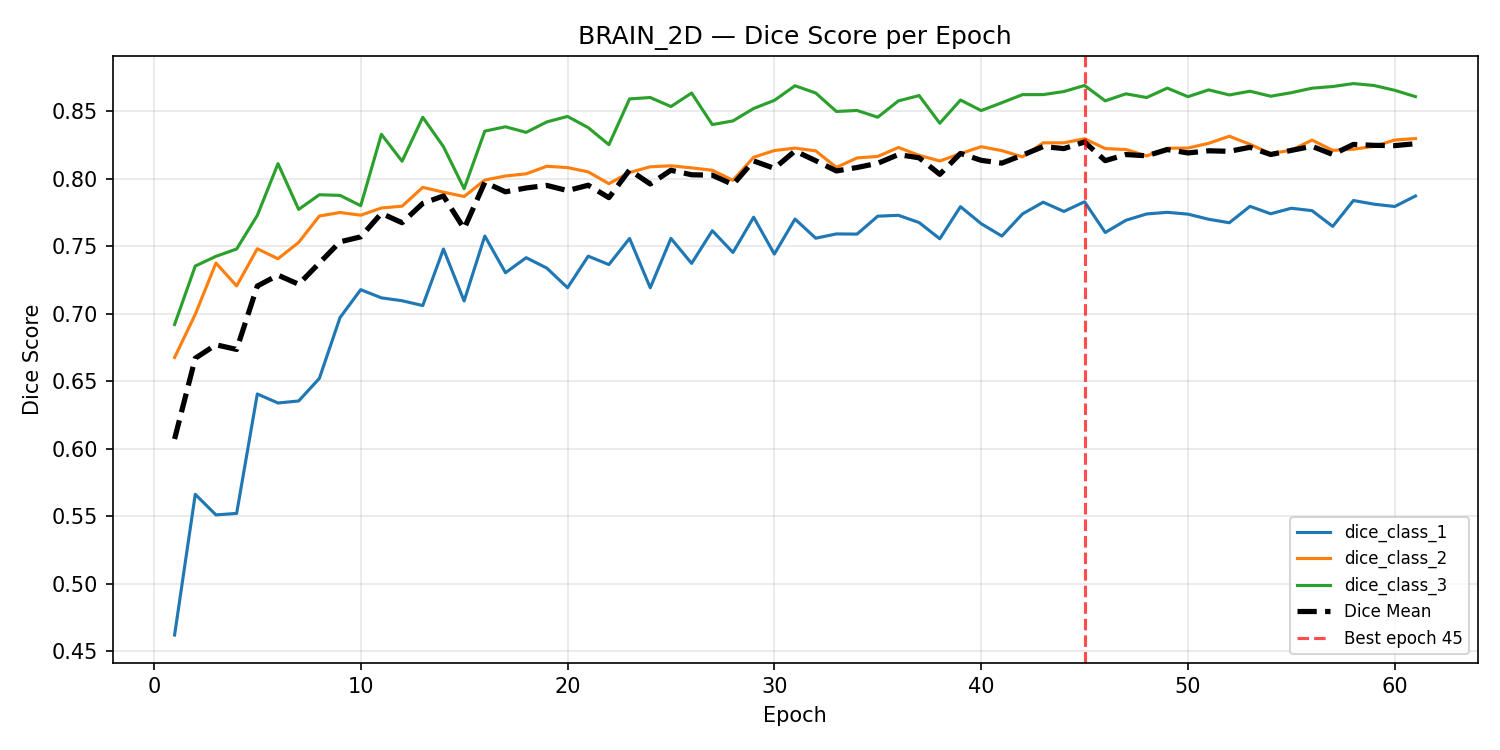
\includegraphics[width=\columnwidth]{figures/brain_2d_dice.png}
  \caption{Beyin 2B Attention U-Net -- dogrulama Dice skorunun epoch'a gore
  degisimi. Ucu sinifta da kararli bir iyilesme var; kontrastlanan tumor
  (yesil) en hizli ogrenilen alt bolge oldu, nekrotik cekirdek (mavi) en
  zoru. En iyi epoch (45) kirmizi dik cizgi ile gosteriliyor.}
  \label{fig:b2d_dice}
\end{figure}

\begin{figure}[!t]
  \centering
  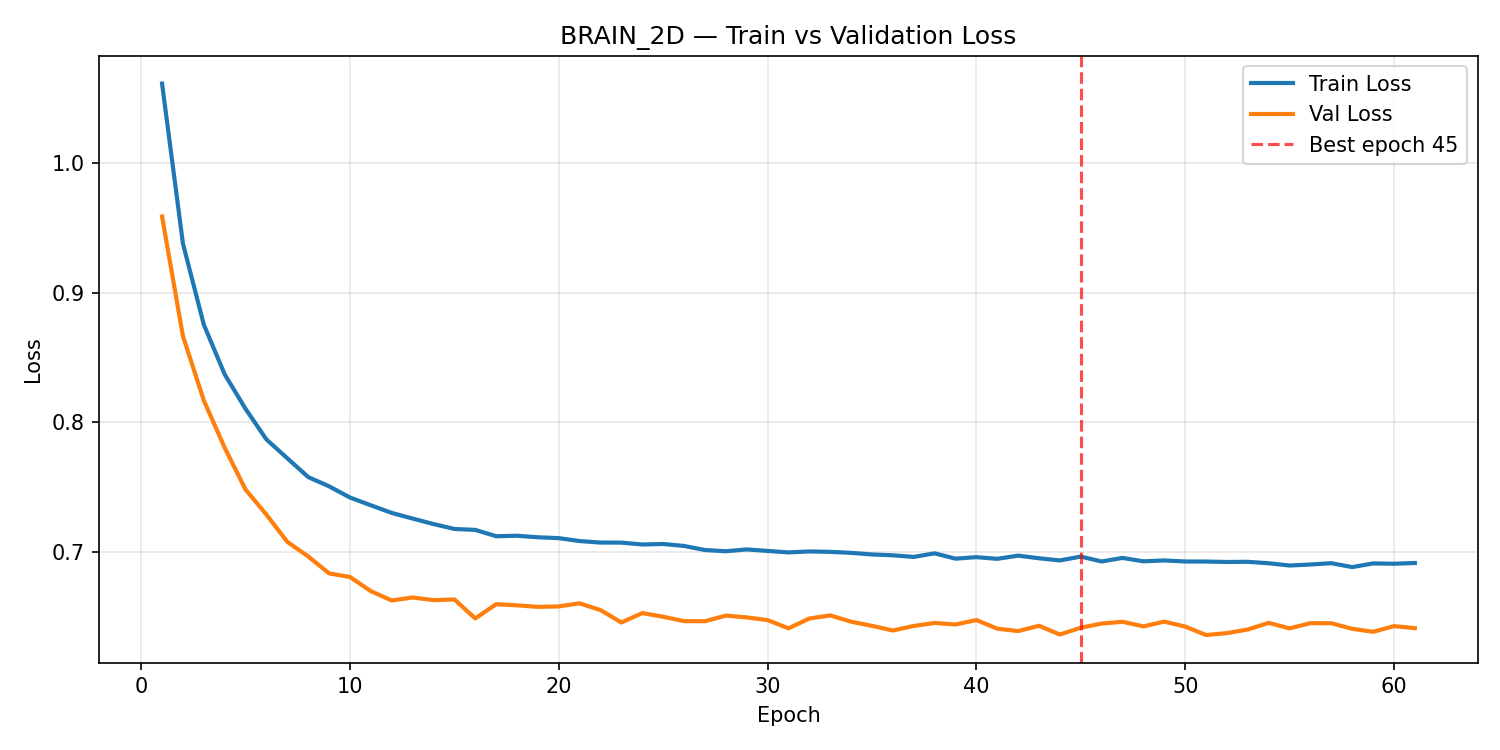
\includegraphics[width=\columnwidth]{figures/brain_2d_loss.png}
  \caption{Beyin 2B -- egitim ve dogrulama yitimi. Egitim yitimi sondaki
  epoch'larda yatay seyrediyor; dogrulama yitiminin de plato yapmasi
  ogrenmenin doygunluga yaklastigini gosterir.}
  \label{fig:b2d_loss}
\end{figure}

\subsection{Beyin MR Segmentasyonu (3B)}

3B model 75 epoch'ta dogrulama Dice'inin yatay seyretmesi uzerine durduruldu.
En iyi epoch 57 idi, \textbf{ortalama Dice 0.764}; sinif bazinda 0.741 / 0.810
/ 0.742 (sirasiyla nekrotik, odem, kontrastlanan). 3B modelin 2B'ye gore daha
dusuk metrik vermesi ilk bakista terslik gibi gorunuyor, ama BraTS gibi
heterojen tumor morfolojilerinde 3B U-Net'in patch boyutuyla ve sliding window
ortusme oranlariyla cok daha hassas oldugu bilinmektedir~\cite{isensee2021nnunet}.
Patch boyutunu artirma denenmedi cunku tek bir 8\,GB VRAM cipi uzerinde
$192^{3}$ patch artik bellege sigmiyordu.

\begin{figure}[!t]
  \centering
  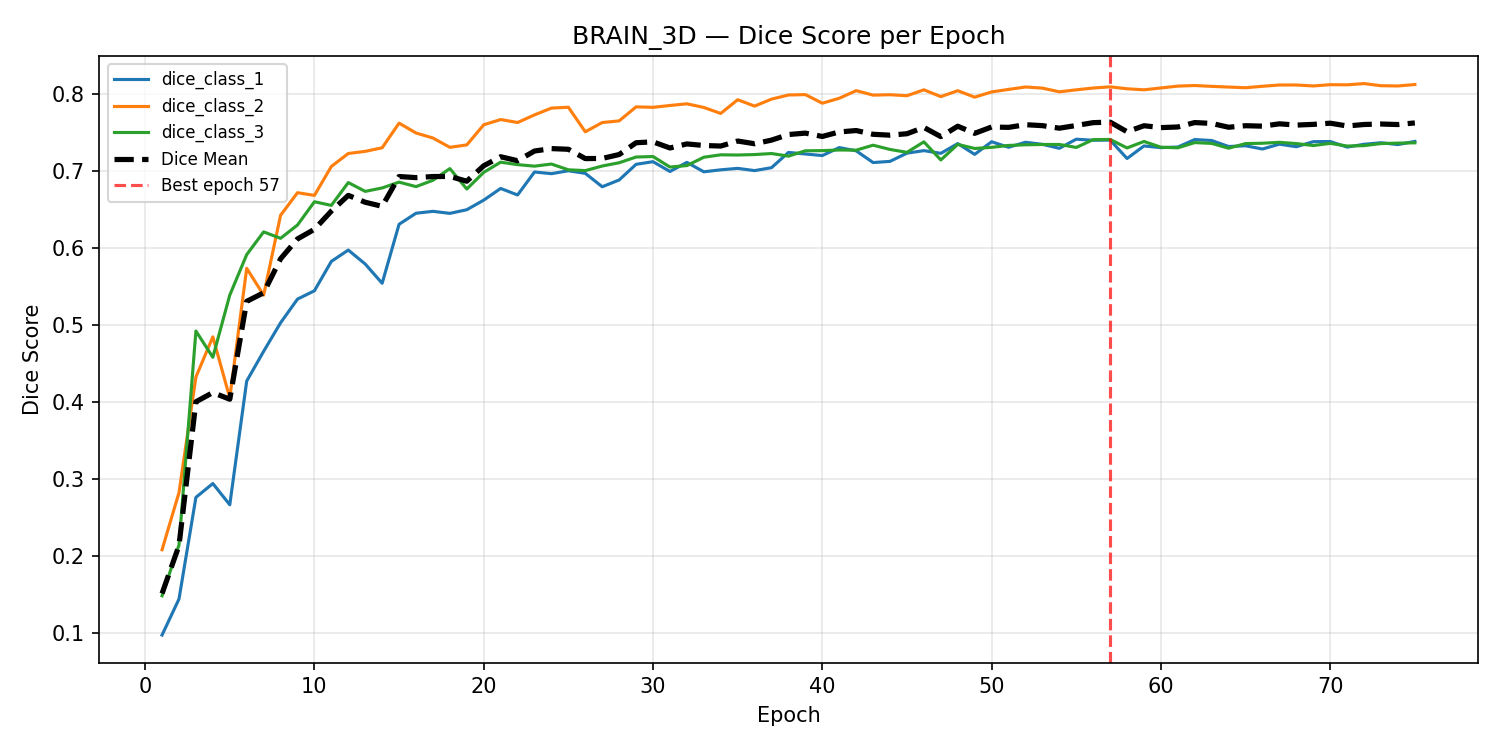
\includegraphics[width=\columnwidth]{figures/brain_3d_dice.png}
  \caption{Beyin 3B Attention U-Net -- dogrulama Dice. Egriler 2B'ye gore
  daha gurultulu, cunku her dogrulama epoch'unda tum hacim sliding window ile
  cikarildigi icin orneklem davranisi daha az duzlestirici.}
  \label{fig:b3d_dice}
\end{figure}

\begin{figure}[!t]
  \centering
  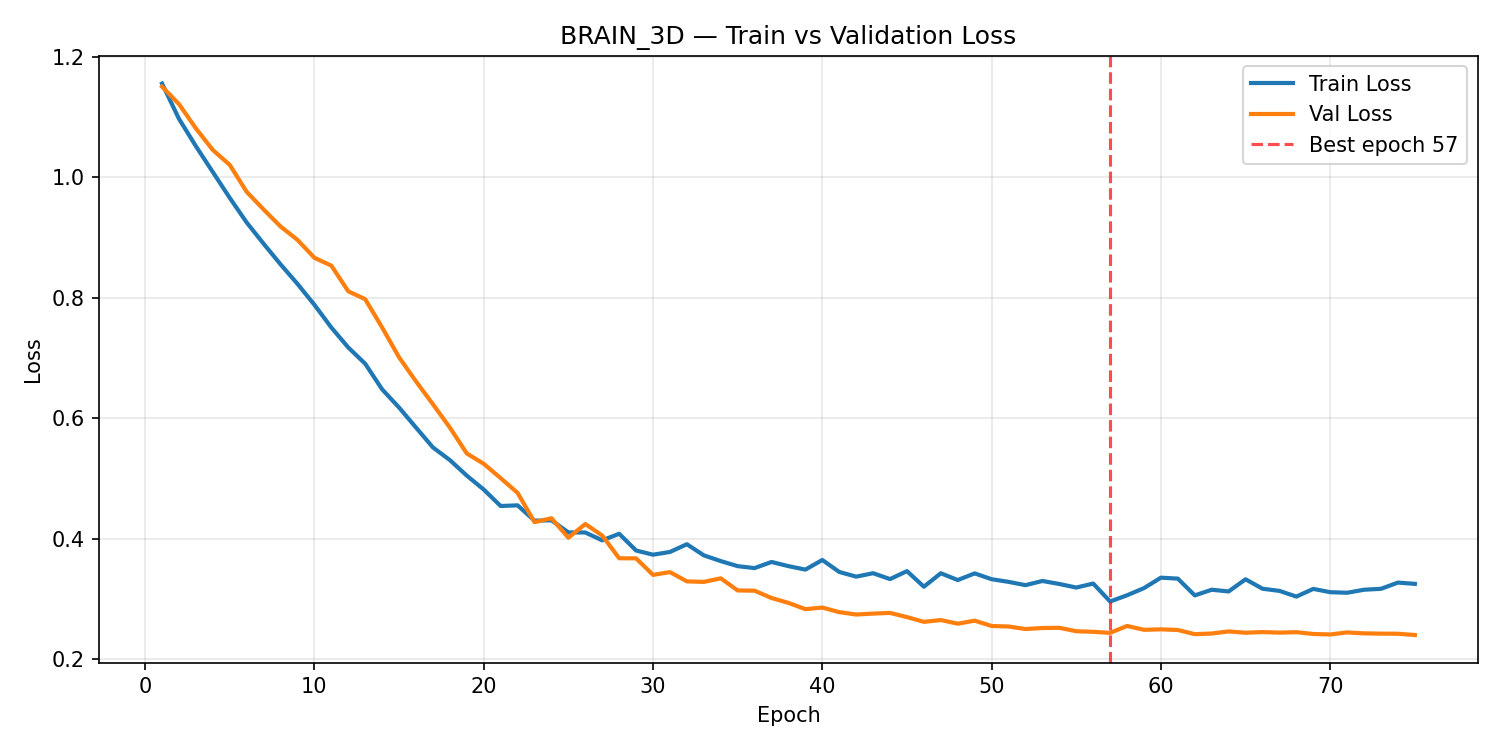
\includegraphics[width=\columnwidth]{figures/brain_3d_loss.png}
  \caption{Beyin 3B -- egitim/dogrulama yitimi. Dogrulama yitimi (turuncu)
  sondaki yaklasik 20 epoch boyunca egitim yitiminin (mavi) altinda; bu, 3B
  patch tabanli artirmanin agresif olmasi, dogrulamanin ise tum hacim
  uzerinde yapilmasi ile aciklanabilir.}
  \label{fig:b3d_loss}
\end{figure}

\subsection{Akciger X-Ray Siniflandirma}

DenseNet-121 modeli 30 epoch'ta erken durdurma ile sonlandi. En iyi epoch 23
idi; dogrulama \textbf{dogrulugu 0.959, makro F1 0.963}. Sinif bazinda F1
skorlari ileri derecede yuksek: COVID 0.982, Lung Opacity 0.936, Normal 0.962,
Viral Pneumonia 0.971 (bkz. Tablo~\ref{tab:lung_f1}).

\begin{table}[!t]
\caption{Akciger siniflandirma -- en iyi epoch (23) sinif bazinda F1}
\label{tab:lung_f1}
\centering
\begin{tabular}{lc}
\toprule
\textbf{Sinif} & \textbf{F1} \\
\midrule
COVID            & 0.982 \\
Lung Opacity     & 0.936 \\
Normal           & 0.962 \\
Viral Pneumonia  & 0.971 \\
\midrule
Makro            & \textbf{0.963} \\
Agirlikli (weighted) & 0.959 \\
Dogruluk         & 0.959 \\
\bottomrule
\end{tabular}
\end{table}

\begin{figure}[!t]
  \centering
  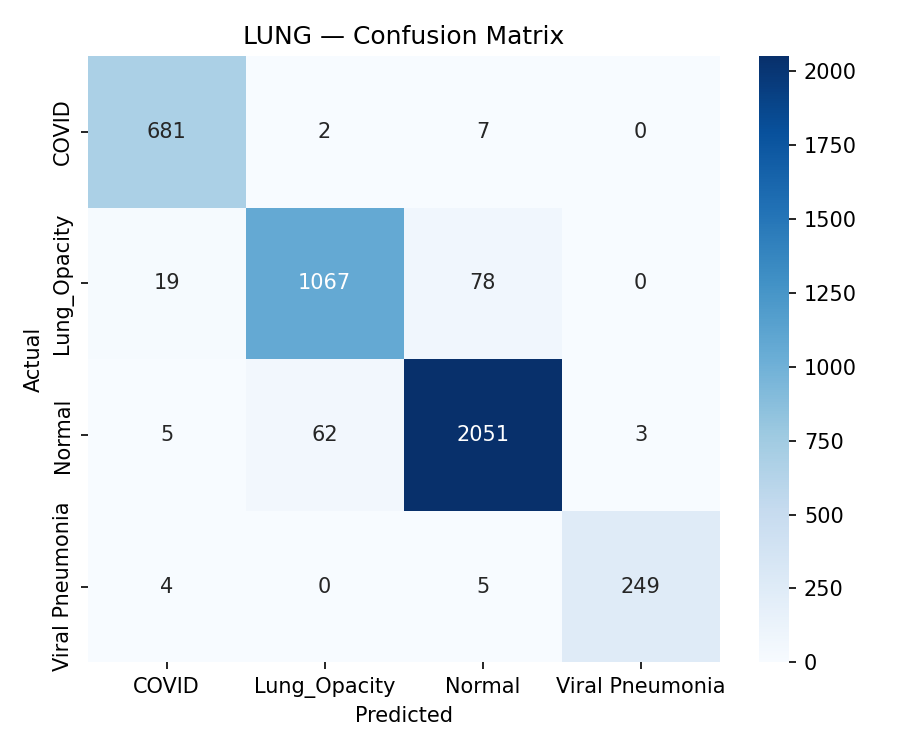
\includegraphics[width=0.95\columnwidth]{figures/lung_confusion.png}
  \caption{Akciger siniflandirma karmasiklik matrisi (dogrulama kumesi).
  Esas hata kaynagi Lung Opacity ile Normal arasindaki karismadir: 78 Lung
  Opacity ornegi Normal olarak, 62 Normal ornegi de Lung Opacity olarak
  siniflandirilmis. Bu, klinik olarak da iki kategorinin sinirinin bulanik
  oldugunu yansitir.}
  \label{fig:lung_cm}
\end{figure}

\begin{figure}[!t]
  \centering
  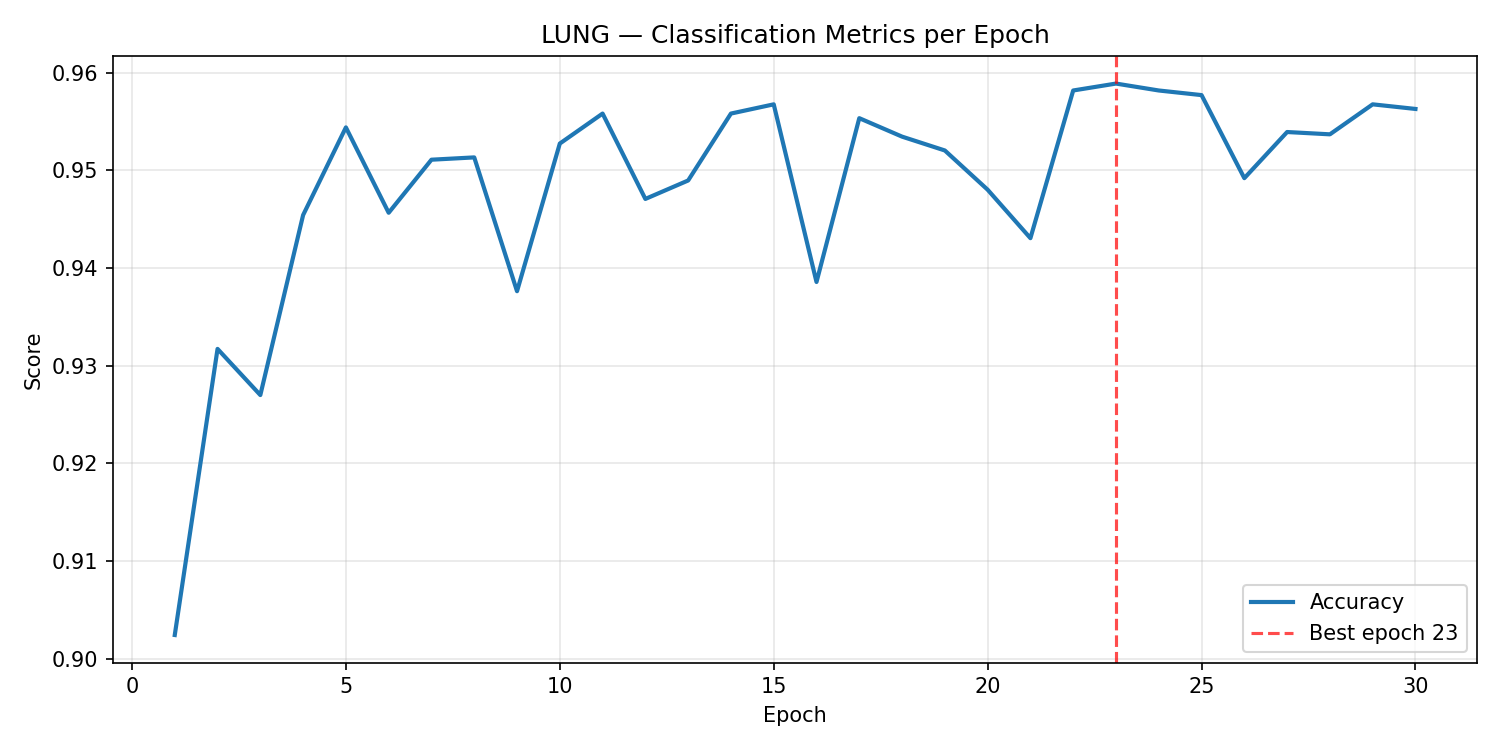
\includegraphics[width=\columnwidth]{figures/lung_accuracy.png}
  \caption{Akciger -- dogrulama dogrulugunun epoch'a gore degisimi. Warm-up'lu
  ogrenme orani plani ilk 5 epoch'ta hizli bir yukselis, ardindan
  CosineAnnealing ile yumusak bir doygunluk ureti.}
  \label{fig:lung_acc}
\end{figure}

\begin{figure}[!t]
  \centering
  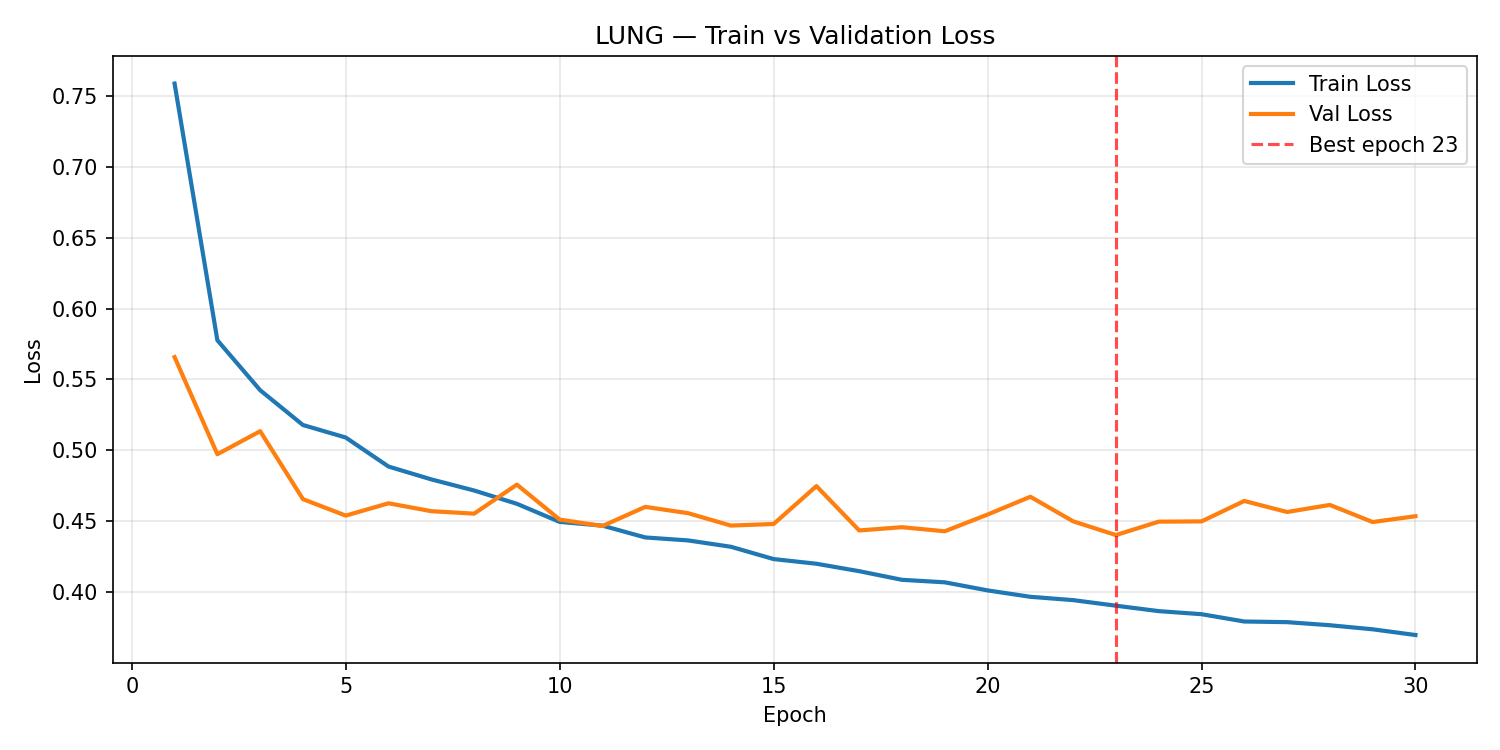
\includegraphics[width=\columnwidth]{figures/lung_loss.png}
  \caption{Akciger -- egitim ve dogrulama yitimi. Yaklasik 10. epoch'tan
  sonra hafif bir asiri ogrenme egilimi var; bu nedenle dogrulama yitiminde 7
  epoch sabir ile erken durdurma kuruldu.}
  \label{fig:lung_loss}
\end{figure}

\subsection{Sonuclarin Kisa Yorumu}

Genel olarak: rontgen siniflandirmasi beklenenden iyi, beyin segmentasyonu
beklendigi seviyede ve 3B model 2B'den dusuk cikti. Akciger taraflanin yuksek
performansi suprize hazirliklisik: COVID-19 Radiography sinin nispeten temiz
ve etiketleri tutarli oldugu icin DenseNet-121 hizla doygunluga ulasti. Beyin
tarafindaki dengesizlik daha cok 3B patch tabanli egitimin ornekleme
hassasiyetinden kaynaklaniyor; 3B'de tek bir patch'in pozitif/negatif orani
modelin gradyanini onemli olcude etkiliyor.

% =============================================================================
\section{Tartisma}

\subsection{Ne Elde Edildi}

Projenin temel hedefi -- yerelde calisan, hicbir verisi dis sunucuya
gondermeden hem segmentasyon hem siniflandirma yapip Turkce bir on rapor
ureten bir tibbi goruntu prototipi -- elde edildi. Spesifik olarak:

\begin{itemize}
  \item BraTS 2020 uzerinde 2B Attention U-Net ile 0.827 ortalama Dice'a
        ulasildi; bu, kucuk olcekli ozel projeler icin makul bir taban cizgisi.
  \item DenseNet-121 ile COVID-19 Radiography uzerinde \%95.9 dogruluk; sinif
        bazinda en zayif F1 yine \%93'un uzerinde.
  \item Grad-CAM ile siniflandirma kararinin neye dayandigi gorsel olarak
        klinisyene gosteriliyor.
  \item Ollama uzerinden Turkce klinik on rapor uretimi; hicbir API anahtari
        gerektirmiyor, tamamen ofline.
  \item Tum sistem PyInstaller ile $\sim$\,4.5\,GB'lik bir
        \texttt{MedicalImagingAI.exe} dosyasina paketlendi; CUDA hizlandirma
        dahil edildi, GPU yoksa otomatik CPU'ya dusuyor.
\end{itemize}

\subsection{Neyi Elde Edemedik, Neden}

\paragraph{3B modelin 2B'yi gecememesi}
Beklentimiz 3B modelin daha dusuk hacimsel bilgi nedeniyle 2B'den belirgin
sekilde ustun olmasiydi. Pratikte 0.064 puanlik bir Dice farkiyla 2B onde
cikti. Asagidaki sebepler etkili oldu:
\begin{itemize}
  \item Sinirli VRAM nedeniyle yalnizca $128^{3}$ patch boyutu kullanilabildi;
        kucuk patch'lerde tumor cevresel baglami kismi sekilde kaybediliyor.
  \item Pozitif/negatif patch orani sabit (1:1) sectik. nnU-Net'in
        \cite{isensee2021nnunet} kullandigi adaptif ornekleme stratejisi
        denenmedi.
  \item Sliding window ortusme orani \%50 idi; %75 daha smooth bir cikti
        verebilirdi ama egitimde dogrulamayi yavaslattigi icin tercih
        edilmedi.
\end{itemize}

\paragraph{Akciger tarafinda baslangic underfitting}
Ilk denemelerimizde model 0.85 dogrulugu asamiyor, ogrenme orani lineer
yukselmis gibi gozukmesine ragmen yitim dususu sabitleniyordu. Su degisiklikler
sirayla denedi:
\begin{enumerate}
  \item \textbf{Donmus on egitim katmanlari}: ilk birkac DenseBlock dondurulmustu;
        ozellik haritalari ImageNet'ten gelmis fotograf gibiydi, X-ray icin
        uygun degildi. \emph{Sonuc:} Tum katmanlarin acilmasi yaklasik
        \%4 dogruluk kazandirdi.
  \item \textbf{Asiri agresif veri artirma}: ilk siralarda MixUp~\cite{zhang2018mixup}
        ve CutMix denedik. Bu, X-ray gibi spatial olarak hassas bir modalitede
        klinik olarak sahte gradyanlar uretti; modelin dogrulama dogrulugu
        epoch'lar arasinda 0.05 puan oynamaya basladi. \emph{Sonuc:} MixUp/CutMix
        kaldirildi, sade flip + rotasyon + parlaklik jitter ile devam edildi.
  \item \textbf{Cosine plani sabit baslangic}: warmup yokken ilk birkac
        epoch'ta loss patladi. Sonra \emph{LinearWarmup}$\!\rightarrow\!$Cosine
        sirasi eklendi: ilk 5 epoch'ta $1\!\times\!10^{-6}\!\rightarrow\!1\!\times\!10^{-4}$,
        ardindan kalan 45 epoch boyunca cosine ile $1\!\times\!10^{-6}$'ya
        inis. \emph{Sonuc:} egitim yitimi ilk epoch'ta dahi kararli kaldi.
\end{enumerate}

Bu adimlar log dosyalarinda izlenebilir; \texttt{results/lung\_metrics.csv}
dosyasi sondaki konfigurasyonun her epoch'unu icerir. Onceki basarisiz
denemelerin egitim ciktilari kasitli olarak repodan cikarilmistir.

\paragraph{Sliding window cikarimi yavasligi}
3B inference sirasinda tek bir hacim CPU'da $\sim$\,60\,s, GPU'da $\sim$\,4\,s
suruyor. Web UI'da bu, kullanicinin "uygulama dondu mu?" hissi vermesine yol
acabiliyor. Asenkron progress bar entegrasyonu yapilmadi.

\paragraph{LLM ciktisi kontrol disi kaliyor}
Ollama \texttt{llama3} ile uretilen Turkce raporlarda zaman zaman uydurma
oranlar (\emph{hallucination}) gozlemlendi, ozellikle hasta yasi/cinsiyeti
verilmediginde. Cikti yapisini kisitlamak icin daha kapsamli prompt
muhendisligi veya bir small/medium Turkce tibbi LLM ince ayari gerekirdi.

\subsection{Kisitlamalar}

Asagidaki kisitlamalar bilinerek dokumantasyona alinmistir. Bu maddeler ayni
zamanda kullanim talimati niteligindedir.

\begin{itemize}
  \item \textbf{Sadece Windows 10/11 64-bit} icin paketleme yapildi. Linux/macOS
        kaynak koddan calistirilabilir, ancak \texttt{.exe} hedefli build
        cross-platform degildir.
  \item Beyin modulu \texttt{.nii} ve \texttt{.nii.gz} (NIfTI) ile DICOM dizini
        kabul eder. Tek bir \texttt{.dcm} dosyasi tek basina yetersizdir, en az
        bir seri klasoru sunulmalidir.
  \item Akciger modulu \texttt{.png} ve \texttt{.jpg} kabul eder; gri tonlu
        rontgenler otomatik olarak 3 kanala kopyalanir.
  \item Modelin BraTS distrubisyonunda olmayan bir MR cihazi/protokolune dair
        belirgin alan kaymasi (\emph{domain shift}) varsa Dice belirgin sekilde
        duser.
  \item LLM rapor uretimi yalnizca Ollama sunucusu \texttt{localhost:11434}
        adresinde calisirken aktif; aksi takdirde sablon tabanli yedek metin
        uretilir.
  \item GPU hizlandirma icin NVIDIA surucusu (CUDA Driver $\ge$ 12.x) gerekir.
        AMD/Intel GPU desteklenmez.
\end{itemize}

\subsection{Calistirma Talimatlari}

Asagidaki adimlar deponun \texttt{README.md} dosyasiyla uyumlu olacak sekilde
ozetlenmistir.

\noindent\textbf{Kaynak koddan calistirma (Windows PowerShell):}
\begin{lstlisting}[language=bash]
git clone https://github.com/BarbarosUmut/Medical_Imaging_Ai.git
cd Medical_Imaging_Ai
python -m venv venv
.\venv\Scripts\Activate.ps1
pip install -r requirements.txt
ollama pull llama3            # bir kez, Ollama'yi ayri kurun
python app/main.py
\end{lstlisting}

\noindent\textbf{Egitim:}
\begin{lstlisting}[language=bash]
python training/train_brain_2d.py     # 2B Attention U-Net
python training/train_brain_3d.py     # 3B Attention U-Net
python training/train_lung.py         # DenseNet-121
\end{lstlisting}

\noindent\textbf{Standalone Windows yurutulebiliri:} Releases sayfasindan
\texttt{MedicalImagingAI-v0.1.0-win64.7z} indirilir, 7-Zip ile acilir ve
\texttt{MedicalImagingAI.exe} calistirilir. Tarayici otomatik olarak
\texttt{http://localhost:7860} adresine acilir.

\subsection{Gelistirme Onerileri}

\paragraph{Daha guclu segmentasyon} Mevcut iskelet \texttt{MONAI AttentionUnet}
uzerinde; nnU-Net~\cite{isensee2021nnunet} cercevesine gecmek hem patch
boyutu/ornekleme sec\-imini hem normalizasyonu otomatize eder. BraTS 2020 test
kumesinde nnU-Net'in bildirilen ortalama Dice degerleri $\geq 0.85$. Bunun
otesinde Swin UNETR~\cite{hatamizadeh2022swinunetr} ve UNETR
~\cite{hatamizadeh2022unetr} gibi transformer omurgali yaklasimlar son iki
BraTS yarismasinda sirasiyla \%4--7 ortalama Dice iyilesmesi raporladi.

\paragraph{Genellestirme} ChestX-ray8~\cite{wang2017chestxray8} veri seti dahil
edilerek dort sinifli model yerine 14 patolojiyi cikti veren bir CheXNet
varyantina~\cite{rajpurkar2017chexnet} gecilebilir. Bu, projeyi tek bir COVID
donemine bagimli olmaktan cikarir.

\paragraph{Yitim fonksiyonu} Sinif dengesizligi belirgin BraTS gibi
goruntulerde Generalised Dice Loss~\cite{sudre2017generalised} ya da Focal
Loss~\cite{lin2017focal} ile DiceCE'nin yer degistirmesi denenebilir.
Ozellikle nekrotik cekirdek gibi gercekten kucuk siniflarda Generalised Dice
iyi sonuclar vermektedir.

\paragraph{LLM tarafi} Mevcut sistem \texttt{llama3} kullaniyor; tibbi alanda
soylem tutarliligi icin Turkce bir tibbi LLM (or. tip-LLM finetune'lari) veya
en azindan Med-PaLM~\cite{singhal2023medpalm} tarzi alan adapte edilmis bir
modelin yerelde kuculmus surumu daha tutarli raporlar uretir.

\paragraph{Kullanici deneyimi} 3B inference icin bir asenkron ilerleme cubugu,
Gradio ile birlestirilebilir; bu, kullanicinin uygulama doniyor mu sorusuna
yanit verir. Ek olarak DICOM serisinin tamamini PACS uzerinden cekme yetenegi
saglanirsa klinik akisin icine yerlestirilebilir.

% =============================================================================
\section{Sonuc}

Bu raporda BraTS 2020 ve COVID-19 Radiography veri setleri uzerinde egitilen
iki segmentasyon ve bir siniflandirma modulunden olusan, yerelde calisan ve
ciktilarini Turkce klinik on rapora doken bir tibbi goruntuleme prototipi
sundum. Performans olarak 2B segmentasyon 0.827, 3B 0.764 ortalama Dice ve
akciger siniflandirmasi 0.963 makro F1 elde etti. Daha onemlisi, raporda
sadece basarilari degil, ilk denemelerde takildigimiz noktalari (donmus
katmanlar, MixUp'in geri cevrilmesi, warm-up ekleme, sliding-window patch
seciminin sinirlari) acikca aktarmaya calistim; bu, ileride benzer projeleri
deneyenler icin uygulama notu olarak daha faydali olur.

Tum kaynak kod, model agirliklari ve standalone Windows derlemesi su adresten
erisilebilir:
\begin{center}
\url{https://github.com/BarbarosUmut/Medical_Imaging_Ai}
\end{center}

% =============================================================================
\section*{Tesekkur}

BraTS 2020 verisi icin organizatorlere~\cite{menze2015brats,bakas2017advancing},
COVID-19 Radiography Database icin Chowdhury vd.~\cite{chowdhury2020covid}
ekibine; ozellikle PyTorch, MONAI~\cite{cardoso2022monai} ve Gradio
gelistiricilerine, ayni zamanda Ollama ekibine yerel LLM calistirma altyapisi
icin tesekkur ederim.

% =============================================================================
\bibliographystyle{IEEEtran}
\bibliography{references}

\end{document}
